\chapter{序論}
深層ニューラルネットワーク(DNN)は,画像認識や自然言語処理など,幅広い分野において著しい性能向上を遂げてきた.特に,ImageNetチャレンジにおける成功を契機に,DNNは視覚的タスクにおいて人間の能力を凌駕する成果を示している\cite{ILSVRC15}.しかし,その性能の背後にある内部表現の形成メカニズムは未だ十分に解明されておらず,その「ブラックボックス」的な性質は重要な研究課題として残されている.モデルの信頼性や透明性を高めるためには,学習プロセスにおける視覚的特徴の獲得メカニズムを明らかにする必要がある.

本研究は,DNNの視覚的特徴の学習プロセスにおいて,特徴獲得の順序や相互作用のメカニズムを明らかにすることを目的とする.特に,学習過程における内部表現の動的変化を系統的に分析するため,新しい実験的枠組みを構築する.視覚的特徴として「数字」と「色」に注目し,データセットを制御することで,学習過程を観察可能な環境を整備する.

本研究では,EMNIST Digitsデータセットに色情報を付加し,視覚的特徴の学習ダイナミクスを解析するための制御可能なデータセットを構築する.これにより,視覚的特徴の学習順序,獲得速度,および特徴間の相互作用を詳細に分析する.学習過程の評価には,モデルの精度を色や数字のみのエラー率に分解し,概念ごとの精度を観察する.
% ,特徴マップの可視化\cite{DBLP:conf/cvpr/ZeilerF14},内部表現のクラスタリング結果など,多角的な評価指標を用いる.

本研究の貢献は以下の3点に要約される.第一に,DNNの学習プロセスを解析するための制御可能な実験環境を構築した.第二に,異なる視覚的特徴の学習順序および相互作用を定量的に評価し,特徴獲得メカニズムを明らかにした.第三に,学習環境におけるノイズの影響を詳細に調査し,モデルのロバスト性と学習効率に関する重要な知見を得た\cite{DBLP:conf/icml/BahdanauCB14}.

これらの成果は,深層学習における内部表現の理解を深めるとともに,効率的かつ解釈可能な学習アルゴリズムの設計に向けた新たな指針を提供するものである.
\newpage
% \begin{figure}[t]
% \centering
% 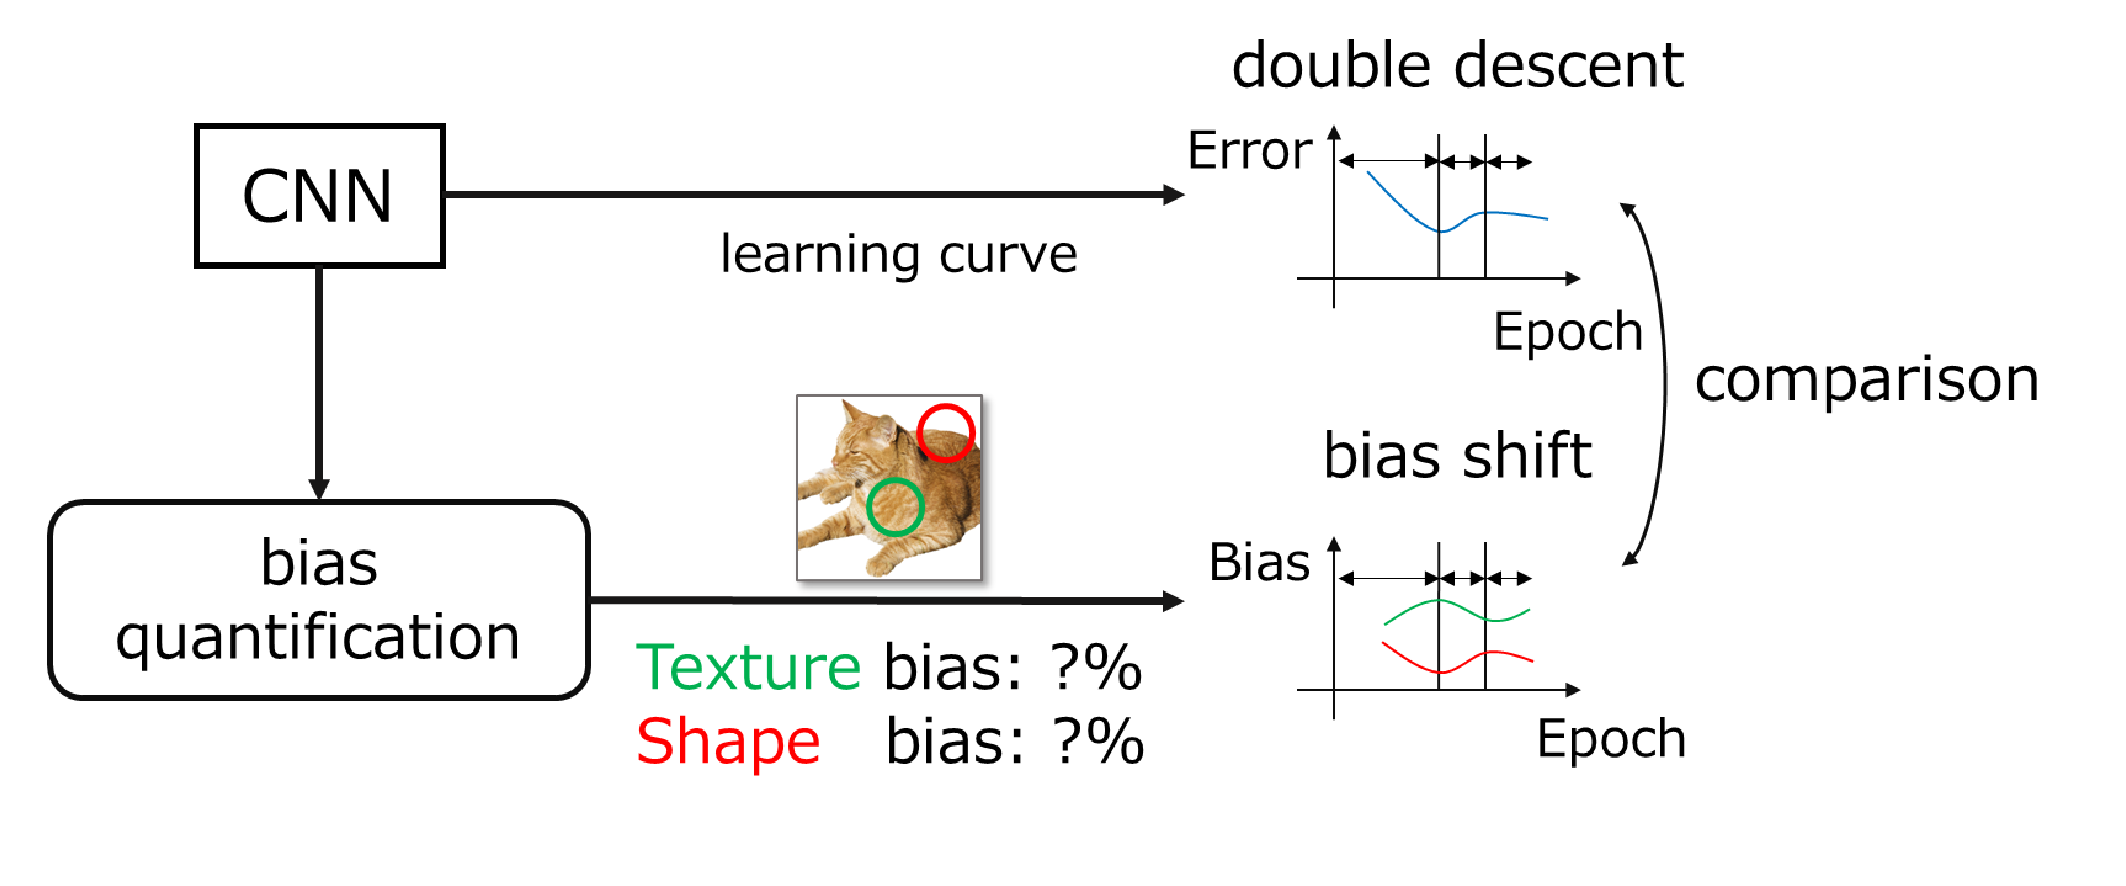
\includegraphics[width=1\columnwidth]{fig/fig1.pdf}
% \vspace{-40pt}
% \caption[ Flow of the analysis process comparing double descent with the learning process of image features.]{
% % 本稿で紹介する解析プロセスの流れ.我々は畳み込みニューラルネットワーク(CNN)を採用し,二重降下条件下で多様な画像認識タスクを訓練した.形状/テクスチャのバイアスとテストエラーの時間的変化を監視し,形状やテクスチャを解釈するモデルの能力を評価すると同時に,それらの相関関係を探った.
% %  Flow of the analysis process comparing double descent with the learning process of image features. We employed convolutional neural networks (CNNs) to train diverse image recognition tasks under double descent conditions. We monitored the temporal evolution of the shape/texture biases and test errors metrics assessing the capacity of the model to interpret shapes and textures while also exploring their correlation.
% }
% \label{fig:fig2}
% \end{figure}

\section{論文構成}
第1章「序論」では,深層学習の急速な発展とその多岐にわたる応用分野について概観し,特に画像認識分野における性能向上とその背景にある主要な技術的進展について述べた.さらに,深層ニューラルネットワーク(DNN)の高い性能を支える内部表現の獲得メカニズムに関する既存の理論的枠組みと,経験的に観測される挙動との間に見られるギャップを指摘し,本研究の対象とする課題の明確化を行った.最後に,DNNの学習プロセスにおける視覚的特徴の獲得順序や相互作用の解明が,モデルの透明性向上や学習効率の改善に寄与することを示し,本研究の目的と貢献点を述べた.\par
第2章「先行研究」では,深層学習における視覚的特徴の獲得の研究がどのように進展してきたかを概観し,特に,画像認識における形状とテクスチャの重要性に関する先行研究を紹介する.さらに,深層学習における重要な経験的に知られる二重降下現象に関する最近の研究成果を紹介し,深層学習の学習プロセスにおける特徴獲得のメカニズムに関する理論的知見と実験的結果を紹介する.\par
第3章「視覚的特徴の獲得を分析するためのデータセット」では,深層学習における,視覚的特徴の獲得メカニズムを紐解くための実験設定を提案し,その設定の理由と目的と述べる.\par
第4章「実験」では,実験手法を詳しく述べる,各種パラメータが与える実験結果への影響について検証する.\par
第5章「結果」では,実験結果を示し,その結果について考察する.\par
第6章「考察」では,実験結果についての考察を行う.\par
第7章「結論」では,本研究を総括する.\par
第8章「今後の展望」では,本研究で得られた知見から今後の方向性を示す.\par
\newpage
